\documentclass{article} % For LaTeX2e
\usepackage{iclr2019_conference,times}

% Optional math commands from https://github.com/goodfeli/dlbook_notation.
\input{math_commands.tex}

\usepackage{amssymb}
\usepackage{hyperref}
\usepackage{url}
\usepackage{graphicx}
\graphicspath{ {./images/} }
\usepackage{listings}

\title{Empirical Comparison of Three Adaptive Moment Optimization Methods}

% Authors must not appear in the submitted version. They should be hidden
% as long as the \iclrfinalcopy macro remains commented out below.
% Non-anonymous submissions will be rejected without review.

\author{Elias Bughsn \\
MSc in Data Science \& Artificial Intelligence \\
Université Côte d'Azur \\
\texttt{eliasbughsn@gmail.com} \\
\And
Quentin Le Roux \\
MSc in Data Science \& Artificial Intelligence \\
Université Côte d'Azur \\
\texttt{quentin.leroux@edhec.com}}

% The \author macro works with any number of authors. There are two commands
% used to separate the names and addresses of multiple authors: \And and \AND.
%
% Using \And between authors leaves it to \LaTeX{} to determine where to break
% the lines. Using \AND forces a linebreak at that point. So, if \LaTeX{}
% puts 3 of 4 authors names on the first line, and the last on the second
% line, try using \AND instead of \And before the third author name.

\newcommand{\fix}{\marginpar{FIX}}
\newcommand{\new}{\marginpar{NEW}}

\iclrfinalcopy % Uncomment for camera-ready version, but NOT for submission.
\begin{document}


\maketitle

\begin{abstract}
Stochastic gradient-based optimization led to the relatively recent development of adaptive 
moment estimation methods, which are known to outperform traditional stochastic gradient-based 
techniques. This paper presents the comparative analysis of three of such methods (i.e. 
Adam, AdamW, and AMSGrad) when applied to industry-standard and real-world datasets in 
the context of a multi-class classification problem.
\end{abstract}

\section{Introduction}

First proposed in 1951, the idea of stochastic approximation revolved around the minimization 
of an objective or risk function with the adjunctive use of noise as part of the optimization 
process \citep{10.1214/aoms/1177729586}:
$$\underset{x}{minimize}\quad F(x) = \mathbb{E}(f(x;\zeta))$$ 

Given $\zeta$ a random seed, and $f(.)$ the composite of a loss function $l$ and a prediction 
function $h$ \citep{bottou2018optimization}. Here the noise represents a random pick from 
the dataset, over which the gradient descent will be performed:
$$\theta = \theta - \eta . \nabla_\theta F(\theta, x^{(i)}, y^{(i)})$$ 

Given $\theta \in \mathbb{R}^d$, the model parameters, $\nabla_\theta F$, the gradient of the 
objective function, $\eta$, the learning rate determining the size of a step taken towards a 
minimum, and $x^{(i)}$ and $y^{(i)}$, a data point and its label respectively in the case
of a classification example.

Overall, stochastic gradient descent (SGD) makes use of practical data in a more efficient 
way than batch methods. Indeed, compared to batch gradient descent, SGD does not perform 
superfluous gradient computations on dataset, which is a concern growing along the size of
computed datasets \citep{ruder2017overview}. Furthermore, the intrinsic randomness allows
the descent to shift towards potentially better minimas. The use of random picks from the 
available data thus enable a more efficient gradient update than when all data is simultaneously 
iterated over. It has been shown that SGD is an efficient method that achieves fast initial 
improvement with low cost \citep{SAvSAA}.

However, standard SGD suffers from the consequence of a static learning rate and its 
inherent noisy fluctuation that impedes the convergence of the descent to the exact, achievable
minimum \citep{inproceedings}. Dealing with this overshooting is a long-standing area of research, 
which led to the recent development of adaptive moment estimation methods.

\section{Adaptive Moment Estimation Methods}
\label{gen_in}

To answer the overshooting problem of standard SGD, development in optimization methods led to 
a foray in how stepsizes are selected at each parameter update during a gradient descent optimization
process. This adaptive approach with regards to the learning parameter found its early expressions 
with the first-order Adaptive Gradient method or AdaGrad \citep{adagrad}, its variant AdaDelta 
\citep{DBLP:journals/corr/abs-1212-5701}, or the unpublished Root Mean Square Propagation or RMSProp
\citep{rms}. While the two former accumulates gradients (all of them for AdaGrad, and a window 
selection for AdaDelta), the latter divides the gradient by a running average over its recent magnitude.

\subsection{Adam}

More recently, an expansion over this concept led to the development of a new kind of optimization
algorithm: the Adaptive Moment Estimation method or Adam \citep{kingma2017adam}. Where the standard 
SGD method keeps a fixed stepsized for all updates, the Adam methods takes inspiration from AdaGrad
and RMSProp. It specifies that the parameter learning rate is updated based on the gradient's first
and second moments and stores an exponentially decaying average of past gradients such that:
$$m_t = \beta_2m_{t-1} + (1-\beta_1)g_t$$
$$v_t = \beta_12v_{t-1} + (1-\beta_1)g^2_t$$
$$\hat{m}_t = \frac{m_t}{1-\beta_1^t}$$
$$\hat{v}_t = \frac{v_t}{1-\beta_2^t}$$
$$\theta_{t+1} = \theta_t - \frac{\eta}{\sqrt{\hat{v}}+\epsilon}\hat{m}_t$$

Given $m_t$, the estimate of the first moment (mean), $v_t$, the estimate of the second moment 
(uncentered variance), and $\hat{m}_t$ and $\hat{v}_t$ their biased-corrected counterparts, 
and $\epsilon$, very small value to avoid dividing by zero. 

With the early success of the method, having shown that it is effective in practice using
large datasets, multiple variants emerged.

\subsection{AdamW}

One such a variant takes advantage of adding a weight decay, resulting in a new algorithm: the
Adam with decoupled weight decay or AdamW \citep{loshchilov2019decoupled}. The idea that spurred
the algorithm's development was the highlight that compared to SGD, $L_2$ regularization and
weight decay were not identical in the case of Adam (For the case of Standard SGD, see the proof
reproduced in Appendix A). As $L_2$ regularization was found not to be as effective 
with Adam, the modification over Adam focused on the update step, inspired from the weight decay
described by \citet{10.5555/2969735.2969756}:
$$\theta_{t+1} = \theta_t - \alpha_t(\frac{\eta\,m_t}{\sqrt{\hat{v}}+\epsilon}+\lambda\theta_{t})$$

Given $\lambda$ the rate of the weight decay at each step and $\alpha_t$ a $SetScheduleMultiplier(t)$
allowing to reset the learning rate during optimization \citep{loshchilov2019decoupled}.

\subsection{AMSGrad}

The final Adaptive Moment Estimation method we are interested in began with the observation of 
a flaw in the Adam method: Adam can fail at converging towards an optimal solution in a convex 
setting \citep{reddi2019convergence}. Indeed, there is an underlying risk that positive definiteness 
could be violated for methods other than Standard SGD.

Given the quantity $\Gamma_t$ measuring the change in the inverse of the learning rate for an 
adaptive method with regards to time such that:
$$\Gamma_{t+1} = \frac{\sqrt{V_{t+1}}}{\eta_{t+1}} - \frac{\sqrt{V_t}}{\eta_t} $$
$$V_t = {diag}(v_t)$$

It happens that for Standard SGD, $\forall t \in [T]\quad \Gamma_t \ge 0$ with $T$, the number 
of rounds. However, this property is not always true for exponential moving average methods such 
as Adam. Indeed, a convex optimization problem like Adam was shown to have a potentially non-zero 
average regret \citep{10.1561/2200000018}, i.e, the delta between the loss of a possible action 
and the action taken given an hypothesis class $h^\star$ would not converge to 
zero \citep{reddi2019convergence}:
$$\frac{R_T}{T} \underset{T\rightarrow\infty}{\nrightarrow} 0$$
$$R_T(h^\star) = \overset{T}{\underset{t=1}{\sum}}l(p_t, y_t) - \overset{T}{\underset{t=1}{\sum}}l(h^\star(x_t), y_t)$$

To remedy to this issue (that the quantity $\Gamma_t$ can be negative for Adam), a new exponential 
moving average method was developed: AMSGrad \citep{reddi2019convergence}. The algorithm is meant 
to guarantee convergence while conserving the advantages of the Adam method. The modification over 
Adam correspond to the computation of $\hat{v}_t$ and of the update step (note the use of $m_t$ 
rather than $\hat{m}_t$) such that:
$$\hat{v}_t = {max}(\hat{v}_{t-1}, v_t)$$
$$\theta_{t+1} = \theta_t-\frac{\eta}{\sqrt{\hat{v}_t}+\epsilon}m_t$$
The main difference with Adam happens with the preserving of the maximum of all past values $v_t$,
which results in never-increasing stepsizes, which was the underlying risk of the Adam method.

\section{Comparison Methodology}
\label{method}

In this section, we present an empirical comparison of the three Adaptive Moment Estimation 
methods we previously covered, using industry-standard and real-world datasets. Our experiments 
will focus on the problem of multi-class classification using various kind of neural networks.

\subsection{Datasets}

Our comparative analysis will rely on three industry-standard fixed-size image datasets: MNIST 
\citep{mnist}, Fashion-MNIST \citep{xiao2017/online}, and CIFAR-10 \citep{cifar}.

The MNIST dataset corresponds to grayscale normalized and centered fixed-size images (28x28 
pixels) of handwritten digits split between 60,000 training and 10,000 testing examples 
respectively. The more recent Fashion-MNIST corresponds to grayscale normalized and centered 
fixed-size images (28x28 pixels) of fashion and clothing articles also split between 60,000 
training and 10,000 testing examples.

Finally, the CIFAR-10 dataset corresponds to color fixed-size images (32x32 pixels with 3 channels) 
split between 50000 training examples and 10000 testing examples, and 10 classes.

Each of those datasets is organized into 10 classes, providing us a standard multi-class 
classification problem. The problem compatibility (image classification on 10 classes) between the 
three datasets allows us to compare Adam, AdamW, and AMSGrad using a variety of interchangeable 
neural network models.

\subsection{Models}

We compare the three Adaptive Moment Estimation methods using four distinct model types: a shallow 
neural network, a deep (fully-connected) neural network, a convolutional neural network, and
a residual neural networks. The graphs for MNIST and Fashion-MNIST can be found in Appendix B, those 
for CIFAR-10 in Appendix C, along with the code in Appendix D.

Each model will use the same suite of hyper-parameters, notably being trained for 100 epochs
with batch sizes of 32 elements with the categorical crossentropy loss. Each optimization 
algorithm will be initialized with default parameters using the TensorFlow library 
\citep{45166}.

\begin{table}[t]
\caption{AdamW and AMSGrad Parameters}
\label{sample-table}
\begin{center}
\begin{tabular}{ll}
\multicolumn{1}{c}{\bf Parameters}  &\multicolumn{1}{c}{\bf Value}
\\ \hline \\
learning rate & $1e^{-2}$ \\
$\beta_1$ & $0.9$ \\
$\beta_2$ & $0.999$ \\
weight decay & $1e^{-4}$ \\
$\epsilon$ & $1e^{-8}$ \\
decay & $0.$
\end{tabular}
\end{center}
\end{table}

\subsection{Comparison approach}

Our comparison approach will be two-fold. We will first take note of the comparative speed of convergence 
between the three different optimizers' losses (for each training session and model). Our second 
approach will be to derive possible ranges of applicability for the optimization algorithms 
based on the models and datasets where they performed the best.

\section{Experiment Results}
\label{results}

The first comparative observation we make relates to the results obtained with the Adam optimization 
algorithm. We can clearly separate the results obtained via Adam from the results obtained 
with AdamW and AMSGrad algorithms as those latter two present similar patterns (See Appendix E for the 
results on the MNIST dataset, Appendix F for the results on the Fashion-MNIST dataset, and
Appendix G for the results on the CIFAR-10 dataset).

A second observation is that, although noisy with the shallow neural network, AdamW and AMSGrad always 
converge quickly for almost all models (the shallow neural network on CIFAR-10 is the outlier, the testing
loss being erratic for all optimizers). However and overall, we can say that, visually, AdamW and AMSGrad
will converge around a mean value in less than 40 epochs. Meanwhile, Adam will converge at a slower pace, 
if not at all (e.g. in the case of the deep neural network, Adam will either result in a increasing loss 
on the testing set, indicating overfitting, or flatline at a high loss value in the case of the CIFAR-10
dataset). Visually, Adam does not seem to reach a convergence point in less than a hundred iterations.

A third observation relates to performance. Although AdamW and AMSGrad converge quickly, they do not 
always achieve a better accuracy result that Adam. Indeed, with most models, Adam ends up achieving 
a better accuracy value on the testing set (See Appendix H for the results on the MNIST dataset, Appendix I 
for the results on the Fashion-MNIST dataset, and Appendix J for the results on the CIFAR-10 dataset).

\section{Conclusion \& Discussion}
\label{discussion}

We saw that the optimizers AdamW and AMSGrad perform better than Adam in the case of convergence in the case
of industry-standard and real-world dataset. In this comparative context, further explorations could be done 
in two regards. 

First, better convergence does not always mean better accuracy results as outlined in the previous section.
A thorough exploration of initialization parameters for AdamW and AMSGrad should be explored so as to see whether
they could match Adam in terms of accuracy performance. Furthermore, new Adaptive Moment Optimization methods
have emerged, and this study could be expanded to cover : Adabound \citep{luo2019adaptive}, Radam 
\citep{liu2020variance}, LAMB \citep{you2020large}, and MAS \citep{landro2020mixing}.

\bibliography{iclr2019_conference}
\bibliographystyle{iclr2019_conference}

\newpage
\appendix
\section{Formal Analysis of Weight Decay vs. $L_2$ Regularization for Standard SGD}
\textbf{Proposition} (Weight decay is equivalent to $L_2$ regularization for standard SGD).
\textit{Standard SGD coupled with a base learning rate $\eta$ executes identical steps between
loss functions $f_t(\theta)$ with a weight decay $\lambda$ and on regularized loss functions
without weight decay $f^{reg}_t(\theta)=f_t(\theta)+\frac{\lambda'}{2}||\theta||^2_2$
with $\lambda'=\frac{\lambda}{\eta}$}.

\textbf{Proof of Proposition} 

The weights update for SGD with regularization and SGD with weight decay are represented
respectively by the following iterates:
$$\theta_{t+1} \leftarrow \theta_t - \eta\nabla f^{reg}_t(\theta_t) = \theta_t - \alpha\nabla f_t(\theta_t) - \eta\lambda'\theta_t$$
$$\theta_{t+1} \leftarrow (1-\lambda)\theta_t - \alpha\nabla f_t(\theta_t)$$

Resulting in the following observation:
$$\lambda' = \frac{\lambda}{\eta}$$

\newpage
\section{Graphs of Neural Networks used for Empirical Comparison For 1-channel images (MNIST and Fashion-MNIST)}

\begin{figure}[h]
\begin{center}
\includegraphics[width=7cm]{images/shallow.png}
\end{center}
\caption{Shallow Neural Network}
\end{figure}

\begin{figure}[h]
\begin{center}
\includegraphics[width=7cm]{images/dnn.png}
\end{center}
\caption{Deep (Fully-Connected) Neural Network}
\end{figure}

\begin{figure}[h]
\begin{center}
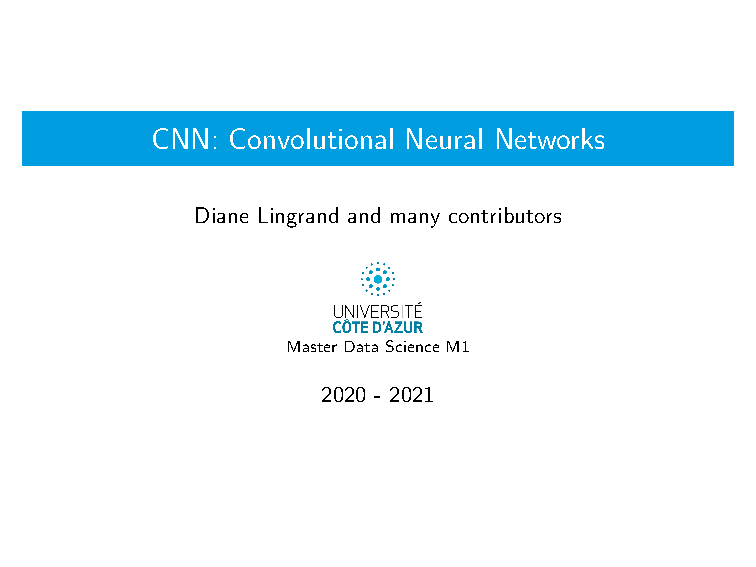
\includegraphics[width=10cm]{images/cnn.png}
\end{center}
\caption{Convolutional Neural Network}
\end{figure}

\begin{figure}[h]
\begin{center}
\includegraphics[width=16cm]{images/resnet.png}
\end{center}
\caption{Residual Neural Network}
\end{figure}

\clearpage
\section{Graphs of Neural Networks used for Empirical Comparison For 3-channel images (CIFAR-10)}

\begin{figure}[h]
\begin{center}
\includegraphics[width=7cm]{images/shallow_3c.png}
\end{center}
\caption{Shallow Neural Network}
\end{figure}

\begin{figure}[h]
\begin{center}
\includegraphics[width=7cm]{images/dnn_3c.png}
\end{center}
\caption{Deep (Fully-Connected) Neural Network}
\end{figure}

\begin{figure}[h]
\begin{center}
\includegraphics[width=10cm]{images/cnn_3c.png}
\end{center}
\caption{Convolutional Neural Network}
\end{figure}

\begin{figure}[h]
\begin{center}
\includegraphics[width=16cm]{images/resnet_3c.png}
\end{center}
\caption{Residual Neural Network}
\end{figure}

\clearpage
\section{Code Implementation using Python and TensorFlow}
\lstset{language=Python}
\lstset{frame=lines}
\lstset{caption={Library Imports}}
\lstset{label={lst:code_direct}}
\lstset{basicstyle=\footnotesize}
\begin{lstlisting}
import matplotlib.pyplot as plt
import numpy as np
import tensorflow as tf

from keras.utils import plot_model, np_utils
from plot_keras_history import plot_history
from tensorflow.keras import Input, Model
from tensorflow.keras.datasets import mnist, fashion_mnist, cifar10
from tensorflow.keras.layers import Flatten, Dense, Concatenate
from tensorflow.keras.layers import Conv2D, SeparableConv2D
from tensorflow.keras.layers import BatchNormalization, Activation
from tensorflow.keras.layers import GlobalAveragePooling2D
from tensorflow.keras.optimizers import Adam
from tensorflow_addons.optimizers import AdamW
\end{lstlisting}

\lstset{language=Python}
\lstset{frame=lines}
\lstset{caption={Custom Function Declarations}}
\lstset{label={lst:code_direct}}
\lstset{basicstyle=\footnotesize}
\begin{lstlisting}
def normalize(dataset):
    """
    Normalizes the pixel values of an image stored as an array
    """
    return dataset/255.

def one_hot_labels(labels):
    """
    One-hot encodes the imported labels
    """
    return tf.one_hot(labels, depth=10)
    
def shallow_neural_network(input_shape, num_classes):
    """
    Creates a shallow neural network
    """
    inputs = Input(shape=input_shape)
    flatten = Flatten()(inputs)
    outputs = Dense(num_classes, activation="softmax")(flatten)
    return Model(inputs, outputs)
    
def deep_neural_network(input_shape, num_classes):
    """
    Creates a Deep (Fully-Connected) Neural Network
    """
    inputs = Input(shape=input_shape)
    flatten = Flatten()(inputs)
    layer_1 = Dense(64, activation="relu")(flatten)
    layer_2 = Dense(32, activation="relu")(layer_1)
    layer_3 = Dense(16, activation="relu")(layer_2)
    outputs = Dense(num_classes, activation="softmax")(layer_3)
    return Model(inputs, outputs)

def convolutional_neural_network(input_shape, num_classes):
    """
    Creates a convolutional neural network
    """
    inputs = Input(shape=input_shape)
    x = Conv2D(128, 3, padding="same", activation="relu")(inputs)
    x = Conv2D(64, 3, padding="same", activation="relu")(x)
    x = Conv2D(32, 3, padding="same", activation="relu")(x)
    x = GlobalAveragePooling2D()(x)
    outputs = Dense(num_classes, activation="softmax")(x)
    return Model(inputs, outputs)
    
def residual_neural_network(input_shape, num_classes):
    """
    Creates a residual neural network
    """
    inputs = Input(shape=input_shape)
    x = Conv2D(128, 3, padding="same", activation="relu")(inputs)
    x = Conv2D(64, 3, padding="same", activation="relu")(x)
    previous_block_activation_1 = x
    previous_block_activation_2 = x
    residual = SeparableConv2D(64, 3, 
                               padding="same", 
                               activation="relu")(previous_block_activation_2)
    x = Concatenate()([x, residual])
    previous_block_activation = x
    residual = SeparableConv2D(64, 3, 
                               padding="same", 
                               activation="relu")(previous_block_activation_1)
    x = Concatenate()([x, residual])
    x = GlobalAveragePooling2D()(x)
    outputs = Dense(num_classes, activation="softmax")(x)
    return Model(inputs, outputs)

def compile_fit(model, X, y, X_val, y_val,
                optimizer, loss, metrics,
                epochs, batch_size):
    """
    Compiles and fits a model given a set of hyperparameters
    """
    model.compile(
        optimizer=optimizer,
        loss=loss,
        metrics=metrics
    )
    history = model.fit(
        x=X, y=y,
        epochs=epochs, batch_size=batch_size,
        validation_data = (X_val, y_val),
        verbose=0
    )
    return history
    
def plot_loss(model, dataset):
    """
    Plots a comparative representation of obtained losses for
    a specific model for all three selected optimizers
    """
    if dataset == "MNIST":
        res = results_mnist
    elif dataset == "Fashion-MNIST":
        res = results_fmnist
    else:
        res = results_cifar
    a = res[f"{model}_adam"].history["loss"]
    b = res[f"{model}_adam"].history["val_loss"]
    c = res[f"{model}_adamw"].history["loss"]
    d = res[f"{model}_adamw"].history["val_loss"]
    e = res[f"{model}_amsgrad"].history["loss"]
    f = res[f"{model}_amsgrad"].history["val_loss"]

    plt.figure(figsize=(12,10))
    plt.plot(a, '--', linewidth=1, color="maroon")
    plt.plot(b, linewidth=3, alpha=0.5, color="firebrick")
    plt.plot(c, '--', linewidth=1, color="lightseagreen")
    plt.plot(d, linewidth=3, alpha=0.5, color="teal")
    plt.plot(e, '--', linewidth=1, color="purple")
    plt.plot(f, linewidth=3, alpha=0.5, color="mediumvioletred")
    plt.xlabel("EPOCHS", fontsize=13)
    plt.ylabel("LOSS VALUE", fontsize=13)
    plt.title("Observed loss values per epoch given " + \
              f"a specific optimizer on the {dataset} dataset",
              fontsize=15)
    plt.legend(["Adam Training Loss", "Adam Testing Loss",
                "AdamW Training Loss", "Adamw Testing Loss",
                "AMSGrad Training Loss", "AMSGrad Testing Loss"],
               fontsize=13)
    plt.show()
\end{lstlisting}

\lstset{language=Python}
\lstset{frame=lines}
\lstset{caption={Dataset Imports}}
\lstset{label={lst:code_direct}}
\lstset{basicstyle=\footnotesize}
\begin{lstlisting}
# 1. Import dataset
# 2. Normalize X arrays (features)
# 3. One-hot encode Y arrays (labels)

# MNIST import
(mx_train, my_train), (mx_test, my_test) = mnist.load_data()
mx_train, mx_test = normalize(mx_train), normalize(mx_test)
my_train, my_test = one_hot_labels(my_train), one_hot_labels(my_test)

# Fashion-MNIST import
(fmx_train, fmy_train), (fmx_test, fmy_test) = fashion_mnist.load_data()
fmx_train, fmx_test = normalize(fmx_train), normalize(fmx_test)
fmy_train, fmy_test = one_hot_labels(fmy_train), one_hot_labels(fmy_test)

# CIFAR-10 import
(cifar_x_train, cifar_y_train), (cifar_x_test, cifar_y_test) = cifar10.load_data()
cifar_x_train = normalize(cifar_x_train)
cifar_x_test = normalize(cifar_x_test)
cifar_y_train = one_hot_labels(cifar_y_train)
cifar_y_test = one_hot_labels(cifar_y_test)
cifar_y_train = tf.reshape(cifar_y_train, [50000, 10])
cifar_y_test = tf.reshape(cifar_y_test, [10000, 10])
\end{lstlisting}

\lstset{language=Python}
\lstset{frame=lines}
\lstset{caption={Model Declarations}}
\lstset{label={lst:code_direct}}
\lstset{basicstyle=\footnotesize}
\begin{lstlisting}
# Global variable declarations
input_shape = (28, 28)
input_shape_cnn = (28, 28, 1)
input_shape_cifar = (32, 32, 3)
num_classes = 10

# Declaring Shallow Models
shallow = shallow_neural_network(input_shape=input_shape, 
                                 num_classes=num_classes)
                                        
# Declaring Deep (Fully-Connected) Models
dnn = deep_neural_network(input_shape=input_shape, 
                          num_classes=num_classes)
                                 
# Declaring Convolutional Models
cnn = convolutional_neural_network(input_shape=input_shape_cnn, 
                                   num_classes=num_classes)

# Declaring ResNet Models
resnet = residual_neural_network(input_shape=input_shape_cnn, 
                                 num_classes=num_classes)
\end{lstlisting}

\lstset{language=Python}
\lstset{frame=lines}
\lstset{caption={Experiments/Computing Loss Results}}
\lstset{label={lst:code_direct}}
\lstset{basicstyle=\footnotesize}
\begin{lstlisting}
# Global variable declarations
epochs = 100
batch_size = 32
loss = "categorical_crossentropy"
metrics = ["accuracy"]

# Generic learning rate and weight decay for AdamW and AMSgrad
lr=0.001
beta_1=0.9
beta_2=0.999
weight_decay=1e-4
epsilon=1e-8
decay=0.

optimizers = [("adam", Adam()), 
              ("adamw", AdamW(lr=lr, beta_1=beta_1, beta_2=beta_2, 
                              weight_decay=weight_decay, epsilon=epsilon, 
                              decay=decay)), 
              ("amsgrad", AdamW(lr=lr, beta_1=beta_1, beta_2=beta_2, 
                                weight_decay=weight_decay, epsilon=epsilon, 
                                decay=decay,
                                amsgrad=True))]

results = {}

# Computes loss results for a kind of model
for name, optimizer in optimizers:
    res = compile_fit(model, 
                      x_train, y_train, 
                      x_test, y_test,
                      optimizer, loss, metrics,
                      epochs, batch_size)
    results[f"{name}"]=res
\end{lstlisting}

\lstset{language=Python}
\lstset{frame=lines}
\lstset{caption={Plotting Results/Data Visualization example with the Shallow model and MNIST dataset}}
\lstset{label={lst:code_direct}}
\lstset{basicstyle=\footnotesize}
\begin{lstlisting}
plot_history(results["f{model}_adam"].history)
plot_history(results["f{model}_adamw"].history)
plot_history(results["f{model}_amsgrad"].history)
plot_loss("f{model}", "f{dataset}")
\end{lstlisting}

\newpage
\section{Observed loss values for each optimizers and models trained on the MNIST dataset}

\begin{figure}[h]
\begin{center}
\includegraphics[width=11cm]{images/mnist_shallow_results.png}
\end{center}
\caption{Results for the shallow neural network trained on MNIST}
\end{figure}

\begin{figure}[h]
\begin{center}
\includegraphics[width=11cm]{images/mnist_deep_results.png}
\end{center}
\caption{Results for the deep neural network trained on MNIST}
\end{figure}

\begin{figure}[h]
\begin{center}
\includegraphics[width=12cm]{images/mnist_cnn_results.png}
\end{center}
\caption{Results for the convolutional neural network trained on MNIST}
\end{figure}

\begin{figure}[h]
\begin{center}
\includegraphics[width=12cm]{images/mnist_resnet_results.png}
\end{center}
\caption{Results for the residual neural network trained on MNIST}
\end{figure}

\clearpage
\section{Observed loss values for each optimizers and models trained on the Fashion-MNIST dataset}

\begin{figure}[h]
\begin{center}
\includegraphics[width=11cm]{images/fmnist_shallow_results.png}
\end{center}
\caption{Results for the shallow neural network trained on Fashion-MNIST}
\end{figure}

\begin{figure}[h]
\begin{center}
\includegraphics[width=11cm]{images/fmnist_deep_results.png}
\end{center}
\caption{Results for the deep neural network trained on Fashion-MNIST}
\end{figure}

\begin{figure}[h]
\begin{center}
\includegraphics[width=12cm]{images/fmnist_cnn_results.png}
\end{center}
\caption{Results for the convolutional neural network trained on Fashion-MNIST}
\end{figure}

\begin{figure}[h]
\begin{center}
\includegraphics[width=12cm]{images/fmnist_resnet_results.png}
\end{center}
\caption{Results for the residual neural network trained on Fashion-MNIST}
\end{figure}

\clearpage
\section{Observed loss values for each optimizers and models trained on the CIFAR-10 dataset}

\begin{figure}[h]
\begin{center}
\includegraphics[width=10.5cm]{images/cifar_shallow_results.png}
\end{center}
\caption{Results for the shallow neural network trained on CIFAR-10}
\end{figure}

\begin{figure}[h]
\begin{center}
\includegraphics[width=10.5cm]{images/cifar_deep_results.png}
\end{center}
\caption{Results for the deep neural network trained on CIFAR-10}
\end{figure}

\begin{figure}[h]
\begin{center}
\includegraphics[width=11cm]{images/cifar_cnn_results.png}
\end{center}
\caption{Results for the convolutional neural network trained on CIFAR-10}
\end{figure}

\begin{figure}[h]
\begin{center}
\includegraphics[width=11cm]{images/cifar_resnet_results.png}
\end{center}
\caption{Results for the residual neural network trained on CIFAR-10}
\end{figure}

\clearpage
\section{Observations of loss and accuracy per model and optimizer for the MNIST dataset}

\begin{figure}[h]
\begin{center}
\includegraphics[width=10.5cm]{images/mnist_shallow_adam.png}
\end{center}
\caption{Loss and accuracy for the shallow neural network with Adam optimizer on MNIST dataset}
\end{figure}

\begin{figure}[h]
\begin{center}
\includegraphics[width=10.5cm]{images/mnist_shallow_adamw.png}
\end{center}
\caption{Loss and accuracy for the shallow neural network with AdamW optimizer on MNIST dataset}
\end{figure}

\begin{figure}[h]
\begin{center}
\includegraphics[width=10.5cm]{images/mnist_shallow_amsgrad.png}
\end{center}
\caption{Loss and accuracy for the shallow neural network with AMSGrad optimizer on MNIST dataset}
\end{figure}

\begin{figure}[h]
\begin{center}
\includegraphics[width=10.5cm]{images/mnist_deep_adam.png}
\end{center}
\caption{Loss and accuracy for the deep neural network Adam optimizer on MNIST dataset}
\end{figure}

\begin{figure}[h]
\begin{center}
\includegraphics[width=10.5cm]{images/mnist_deep_adamw.png}
\end{center}
\caption{Loss and accuracy for the deep neural network with AdamW optimizer on MNIST dataset}
\end{figure}

\begin{figure}[h]
\begin{center}
\includegraphics[width=10.5cm]{images/mnist_deep_amsgrad.png}
\end{center}
\caption{Loss and accuracy for the deep neural network with AMSGrad optimizer on MNIST dataset}
\end{figure}

\begin{figure}[h]
\begin{center}
\includegraphics[width=10.5cm]{images/mnist_cnn_adam.png}
\end{center}
\caption{Loss and accuracy for the convolutional neural network with Adam optimizer on MNIST dataset}
\end{figure}

\begin{figure}[h]
\begin{center}
\includegraphics[width=10.5cm]{images/mnist_cnn_adamw.png}
\end{center}
\caption{Loss and accuracy for the convolutional neural network with AdamW optimizer on MNIST dataset}
\end{figure}

\begin{figure}[h]
\begin{center}
\includegraphics[width=10.5cm]{images/mnist_cnn_amsgrad.png}
\end{center}
\caption{Loss and accuracy for the convolutional neural network with AMSGrad optimizer on MNIST dataset}
\end{figure}

\begin{figure}[h]
\begin{center}
\includegraphics[width=10.5cm]{images/mnist_resnet_adam.png}
\end{center}
\caption{Loss and accuracy for the residual neural network with Adam optimizer on MNIST dataset}
\end{figure}

\begin{figure}[h]
\begin{center}
\includegraphics[width=10.5cm]{images/mnist_resnet_adamw.png}
\end{center}
\caption{Loss and accuracy for the residual neural network with AdamW optimizer on MNIST dataset}
\end{figure}

\begin{figure}[h]
\begin{center}
\includegraphics[width=10.5cm]{images/mnist_resnet_amsgrad.png}
\end{center}
\caption{Loss and accuracy for the residual neural network with AMSGrad optimizer on MNIST dataset}
\end{figure}

\clearpage
\section{Observations of loss and accuracy per model and optimizer for the Fashion-MNIST dataset}

\begin{figure}[h]
\begin{center}
\includegraphics[width=10.5cm]{images/fmnist_shallow_adam.png}
\end{center}
\caption{Loss and accuracy for the shallow neural network with Adam optimizer on Fashion-MNIST dataset}
\end{figure}

\begin{figure}[h]
\begin{center}
\includegraphics[width=10.5cm]{images/fmnist_shallow_adamw.png}
\end{center}
\caption{Loss and accuracy for the shallow neural network with AdamW optimizer on Fashion-MNIST dataset}
\end{figure}

\begin{figure}[h]
\begin{center}
\includegraphics[width=10.5cm]{images/fmnist_shallow_amsgrad.png}
\end{center}
\caption{Loss and accuracy for the shallow neural network with AMSGrad optimizer on Fashion-MNIST dataset}
\end{figure}

\begin{figure}[h]
\begin{center}
\includegraphics[width=10.5cm]{images/fmnist_deep_adam.png}
\end{center}
\caption{Loss and accuracy for the deep neural network Adam optimizer on Fashion-MNIST dataset}
\end{figure}

\begin{figure}[h]
\begin{center}
\includegraphics[width=10.5cm]{images/fmnist_deep_adamw.png}
\end{center}
\caption{Loss and accuracy for the deep neural network with AdamW optimizer on Fashion-MNIST dataset}
\end{figure}

\begin{figure}[h]
\begin{center}
\includegraphics[width=10.5cm]{images/fmnist_deep_amsgrad.png}
\end{center}
\caption{Loss and accuracy for the deep neural network with AMSGrad optimizer on Fashion-MNIST dataset}
\end{figure}

\begin{figure}[h]
\begin{center}
\includegraphics[width=10.5cm]{images/fmnist_cnn_adam.png}
\end{center}
\caption{Loss and accuracy for the convolutional neural network with Adam optimizer on Fashion-MNIST dataset}
\end{figure}

\begin{figure}[h]
\begin{center}
\includegraphics[width=10.5cm]{images/fmnist_cnn_adamw.png}
\end{center}
\caption{Loss and accuracy for the convolutional neural network with AdamW optimizer on Fashion-MNIST dataset}
\end{figure}

\begin{figure}[h]
\begin{center}
\includegraphics[width=10.5cm]{images/fmnist_cnn_amsgrad.png}
\end{center}
\caption{Loss and accuracy for the convolutional neural network with AMSGrad optimizer on Fashion-MNIST dataset}
\end{figure}

\begin{figure}[h]
\begin{center}
\includegraphics[width=10.5cm]{images/fmnist_resnet_adam.png}
\end{center}
\caption{Loss and accuracy for the residual neural network with Adam optimizer on Fashion-MNIST dataset}
\end{figure}

\begin{figure}[h]
\begin{center}
\includegraphics[width=10.5cm]{images/fmnist_resnet_adamw.png}
\end{center}
\caption{Loss and accuracy for the residual neural network with AdamW optimizer on Fashion-MNIST dataset}
\end{figure}

\begin{figure}[h]
\begin{center}
\includegraphics[width=10.5cm]{images/fmnist_resnet_amsgrad.png}
\end{center}
\caption{Loss and accuracy for the residual neural network with AMSGrad optimizer on Fashion-MNIST dataset}
\end{figure}

\clearpage
\section{Observations of loss and accuracy per model and optimizer for the CIFAR-10 dataset}

\begin{figure}[h]
\begin{center}
\includegraphics[width=10.5cm]{images/cifar_shallow_adam.png}
\end{center}
\caption{Loss and accuracy for the shallow neural network with Adam optimizer on CIFAR-10 dataset}
\end{figure}

\begin{figure}[h]
\begin{center}
\includegraphics[width=10.5cm]{images/cifar_shallow_adamw.png}
\end{center}
\caption{Loss and accuracy for the shallow neural network with AdamW optimizer on CIFAR-10 dataset}
\end{figure}

\begin{figure}[h]
\begin{center}
\includegraphics[width=10.5cm]{images/cifar_shallow_amsgrad.png}
\end{center}
\caption{Loss and accuracy for the shallow neural network with AMSGrad optimizer on CIFAR-10 dataset}
\end{figure}

\begin{figure}[h]
\begin{center}
\includegraphics[width=10.5cm]{images/cifar_deep_adam.png}
\end{center}
\caption{Loss and accuracy for the deep neural network Adam optimizer on CIFAR-10 dataset}
\end{figure}

\begin{figure}[h]
\begin{center}
\includegraphics[width=10.5cm]{images/cifar_deep_adamw.png}
\end{center}
\caption{Loss and accuracy for the deep neural network with AdamW optimizer on CIFAR-10 dataset}
\end{figure}

\begin{figure}[h]
\begin{center}
\includegraphics[width=10.5cm]{images/cifar_deep_amsgrad.png}
\end{center}
\caption{Loss and accuracy for the deep neural network with AMSGrad optimizer on CIFAR-10 dataset}
\end{figure}

\begin{figure}[h]
\begin{center}
\includegraphics[width=10.5cm]{images/cifar_cnn_adam.png}
\end{center}
\caption{Loss and accuracy for the convolutional neural network with Adam optimizer on CIFAR-10 dataset}
\end{figure}

\begin{figure}[h]
\begin{center}
\includegraphics[width=10.5cm]{images/cifar_cnn_adamw.png}
\end{center}
\caption{Loss and accuracy for the convolutional neural network with AdamW optimizer on CIFAR-10 dataset}
\end{figure}

\begin{figure}[h]
\begin{center}
\includegraphics[width=10.5cm]{images/cifar_cnn_amsgrad.png}
\end{center}
\caption{Loss and accuracy for the convolutional neural network with AMSGrad optimizer on CIFAR-10 dataset}
\end{figure}

\begin{figure}[h]
\begin{center}
\includegraphics[width=10.5cm]{images/cifar_resnet_adam.png}
\end{center}
\caption{Loss and accuracy for the residual neural network with Adam optimizer on CIFAR-10 dataset}
\end{figure}

\begin{figure}[h]
\begin{center}
\includegraphics[width=10.5cm]{images/cifar_resnet_adamw.png}
\end{center}
\caption{Loss and accuracy for the residual neural network with AdamW optimizer on CIFAR-10 dataset}
\end{figure}

\begin{figure}[h]
\begin{center}
\includegraphics[width=10.5cm]{images/cifar_resnet_amsgrad.png}
\end{center}
\caption{Loss and accuracy for the residual neural network with AMSGrad optimizer on CIFAR-10 dataset}
\end{figure}

\end{document}